\newpage
\section{SIMULADORES} \label{simuladores}

Ante el creciente interés internacional por el empleo de la energía nuclear para satisfacer las grandes necesidades energéticas a las que se enfrenta la sociedad actual, la educación y formación de personal cualificado son cruciales para garantizar la operación segura y fiable de las centrales nucleares. Los simuladores para la educación y formación nuclear son una herramienta muy efectiva para el aprendizaje de múltiples habilidades y conocimientos necesarios tanto en el ámbito académico como profesional del sector nuclear.

Los avances en la tecnología informática han permitido el desarrollo de simuladores de alta precisión y fiabilidad tanto a escala real como a escalas más pequeñas y simples. Los simuladores más simples, en comparación con los simuladores de alcance total, permiten a los aprendices captar más rápidamente los fundamentos de operación mediante el aprendizaje práctico, sin perder igualmente los detalles de los complejos procesos tecnológicos de la planta. La combinación de la instrucción teórica sobre la física y la tecnología nuclear, junto con el aprendizaje práctico mediante la experiencia en un simulador, ha demostrado ser un método de aprendizaje avanzado y efectivo que fortalece la comprensión de los principios fundamentales de la tecnología nuclear. 

Las diferencias en el alcance, los modelos de simulación, las interfaces del instructor y del aprendiz y otras muchas características, permiten el uso de estos simuladores para la formación de una amplia variedad de personal. Muchas necesidades educativas y de formación técnica pueden ser atendidas utilizando varios tipos de simuladores orientados a objetivos instructivos específicos.

\subsection{Tipos de simuladores}

En primer lugar, es importante tener en cuenta los siguientes dos grandes objetivos generales del empleo de estos simuladores:

\begin{enumerate}
  \item \underline{Educación nuclear:} Adquisición de conocimientos para la comprensión detallada de los conceptos, fenómenos y tecnologías relacionados con la energía nuclear.
  \item \underline{Formación nuclear:} Desarrollo de capacidades para la mejora de las habilidades, actitudes y comportamientos dentro del entorno específico de una central nuclear.
\end{enumerate}

En base a las definiciones anteriores, el \acrshort{oiea} clasifica los simuladores de reactores nucleares en los siguientes tipos:

\begin{enumerate}
  \item \underline{Simuladores básicos de educación y formación:} Comúnmente denominados simuladores de principios básicos, tienen como principal objetivo ayudar a los usuarios a comprender los procesos físicos fundamentales, la operación básica, el diseño de sistemas y los procedimientos operativos generales de las centrales nucleares. Estos simuladores no están vinculados necesariamente a una central nuclear concreta, sino a un tipo de diseño de reactor específico (\acrshort{pwr}, \acrshort{bwr}, \acrfull{candu}, reactores avanzados, etc.). Son ampliamente utilizados en programas de educación básica y superior, y pueden ser de dos tipos:
  \begin{itemize}
    \item \textbf{Simuladores de tareas parciales:} Abordan una parte específica de las operaciones de la planta, centrándose en sistemas, componentes o fenómenos concretos (por ejemplo, en la ruptura de tubos del generador de vapor o en el arranque y operación de los generadores diésel...). Se emplean cuando se desea facilitar el aprendizaje en aspectos muy concretos.
    
    \item \textbf{Simuladores de planta completa:} Ofrecen una visión general del comportamiento de la central nuclear, con un enfoque en los sistemas principales, con o sin los sistemas auxiliares. Se emplean cuando se desea proporcionar una comprensión general del comportamiento de la planta y los procesos principales (por ejemplo, el comportamiento en estado estable o transitorio de la planta, el sistema refrigeración del reactor, el sistema de vapor principal...).
  \end{itemize}
  \item \underline{Simuladores de formación profesional:} Abordan la totalidad de componentes y sistemas de la planta; sus funciones, procesos de operación integrales y los efectos internos en múltiples parámetros del sistema durante la operación en condiciones normales, transitorias y de accidente. Abarcan, a su vez, cuatro tipologías distintas de simuladores:
  \begin{itemize}
    \item \textbf{Simuladores de aula específicos de la planta:} Son simuladores con paneles virtuales y/o una interfaz del operador (sin paneles de hardware). Los gráficos se muestran en monitores estándar, monitores táctiles o pantallas proyectadas. El alcance de modelado de este tipo de simuladores es similar al de un simulador de alcance total, pero sin los paneles físicos, consolas e instrumentos asociados. La profundidad y fidelidad del modelado no necesariamente es tan alta como la de un simulador de alcance total. Para estos simuladores, el modelado de procesos en tiempo real puede no ser requerido. Pueden ser, a su vez, de dos tipos:
    \begin{itemize}
      \item \textbf{Simuladores de tareas parciales:} Como se ha comentado anteriormente, simulan componentes, sistemas y fenómenos específicos de la planta.
      \item \textbf{Simuladores de planta completa:} Simulan la el comportamiento de la planta en su totalidad tanto en condiciones de operación normal como en transitorios o accidentes.
    \end{itemize}
    \item \textbf{Simuladores de mantenimiento o de componentes:} Se centran en capacitar al personal para la realización de tareas relacionadas con componentes o sistemas muy específicos de la planta, como el ensamblaje y desensamblaje de componentes o la operación de una máquina de recarga de combustible. Para estos simuladores, no se requiere el modelado de procesos en tiempo real.
    \item \textbf{Simuladores de ingeniería:} Simuladores en tiempo real utilizados para demostrar el comportamiento de una central nuclear en operación normal, transitorios o accidentes con más detalle que los simuladores básicos de educación y formación. Se utilizan principalmente para la optimización del diseño de la planta y la generación de documentos de Análisis de Seguridad de la Planta. También pueden ser utilizados para la formación profesional del personal de la central sobre la dinámica de la planta y la comprensión de escenarios o condiciones de accidentes severos en relación con los límites de seguridad del diseño.
    \item \textbf{Simuladores de alcance total:} Se trata de herramientas muy potentes vinculadas a una central nuclear concreta. Operan en tiempo real y se utilizan principalmente para la licencia de operadores y para la formación de otros empleados de la central. Su objetivo es desarrollar los conocimientos, las habilidades, los reflejos y las actitudes necesarias para demostrar su capacitación para operar la central nuclear de forma segura. Constan de un modelo matemático completo de todos los sistemas y modos de operación de la central. Pueden ser de réplica exacta de la sala de control principal de la central nuclear en cuestión o gráficos interactivos, análogos a los anteriores, pero totalmente operados mediante ordenadores (\cite{international2019iaea}).
  \end{itemize}
\end{enumerate}

En el siguiente diagrama, se muestra de forma visual la clasificación anteriormente explicada de forma detallada:

\begin{figure}[h]
  \centering
  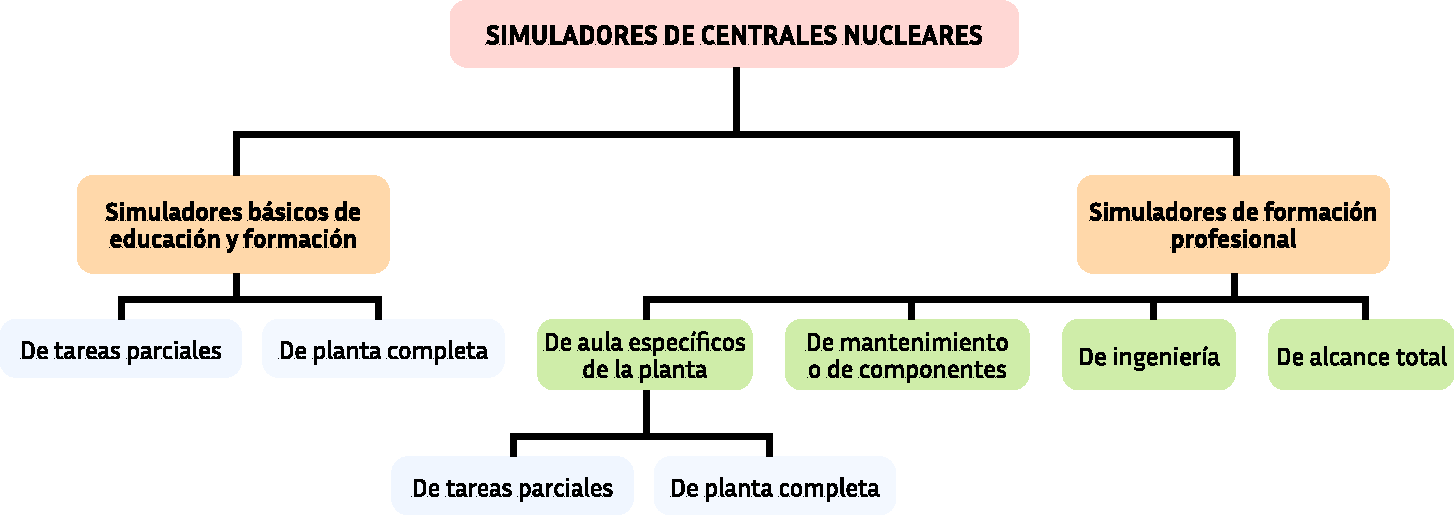
\includegraphics[width=\textwidth]{content/figures/clasificacion_simuladores.pdf}
  \caption{Clasificación de los simuladores de centrales nucleares (\cite{international2019iaea}).}
  \label{fig:clasificacion_simuladores}
\end{figure}

\subsection{Simuladores de SMRs}

Debido al papel fundamental que tienen los \acrshortpl{smr} en la transición energética de múltiples países del mundo, se han desarrollado ---y se siguen desarrollando--- simuladores para la formación específica en estos reactores avanzados. La filosofía de estos simuladores es análoga a la de los simuladores de las centrales nucleares convencionales, solo que incluyen las propiedades, sistemas, componentes y  modos de operación avanzados correspondientes. Además, al ser más recientes, se diseñan con los códigos, algoritmos, modelos y métodos de simulación y computación más actualizados posibles. 

A continuación, se exponen brevemente dos ejemplos destacables: el \textit{E2 Center} y los simuladores de \acrshortpl{smr} de Tecnatom ---simuladores básicos de educación de planta completa---. Aun así, existen muchos otros simuladores de este tipo, como el \textit{BWRX-300 Simulator} de Hitachi, el \textit{SMART Reactor Simulator}, el simulador de \textit{Terrapower} y otros simuladores desarrollados por empresas especializadas en simulación industrial, como \textit{CORYS} o \textit{L3Harris}, entre otras.

\subsubsection{E2 Center}

El \textit{E2 Center} es un entorno de aprendizaje innovador que emplea un modelado informático de última generación para la simulación de la sala de control del VOYGR-12, un \acrlong{smr} de 12 unidades de 77 MWe cada una (total de 924 MWe), desarrollado por NuScale.

El sistema consta de múltiples interfaces que permiten a los operadores de la sala de control ingresar múltiples parámetros, ejecutar una variedad de escenarios y observar la consecuente respuesta de la central. Cada estación de trabajo puede ver el estado de cualquiera de las 12 unidades que componen la planta. Asimismo, presenta características avanzadas de automatización que facilitan el control de la central por parte de los operadores, y muestran de forma muy visual los avisos, alarmas y procedimientos a seguir tanto en operación normal como en transitorios.

NuScale se encarga de la construcción e instalación del centro, proporciona un manual de usuario y una guía de ejercicios para el cliente, y brinda el soporte técnico necesario. Actualmente, este simulador se ha implementado en 6 ubicaciones distintas: 4 pertenecientes a EEUU, una en Bucarest (Rumanía) y otra en Seúl (Corea del Sur).

\begin{figure}[h!]
  \centering
  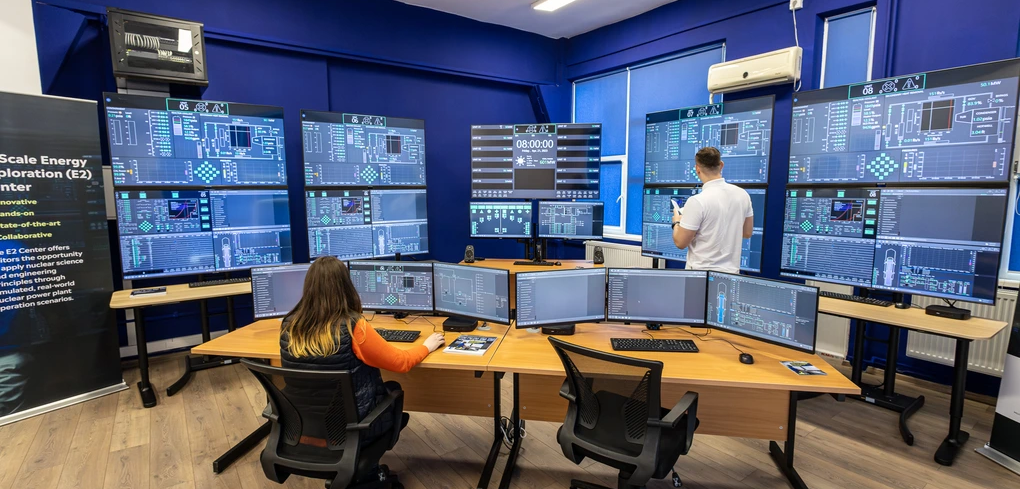
\includegraphics[width=0.75\textwidth]{content/figures/e2_center_bucarest.png}
  \caption{E2 Center de la Universidad Politécnica de Bucarest (\cite{e2_center_romania}).}
  \label{fig:e2_center_bucarest}
\end{figure}

\subsubsection{Simuladores de SMRs de Tecnatom}

En 2017, Tecnatom desarrolló un simulador de \acrshortpl{smr} de tipo \acrshort{pwr}, denominados \acrfullpl{ipwr}, en los que todos los componentes del circuito primario se encuentran integrados en el interior de la vasija del reactor, tal y como se detalla en el apartado \ref{seguridad}. Se trata de un simulador \textit{online} de descarga gratuita bajo licencia del \acrshort{oiea} en el que, a parte de familiarizarse con la arquitectura integral del reactor, el usuario puede poner a prueba los distintos sistemas de seguridad avanzados de los que dispone el reactor ---la mayoría de ellos pasivos---, mediante la simulación de múltiples tipos de accidentes distintos (\cite{ipwr_iaea}).

Actualmente, Tecnatom está desarrollando un simulador de \acrshort{smr} para el \textit{Institute of Energy Technology (IFE)} de Noruega, con el objetivo de posibilitar la operación y la monitorización de una sala de control multiunidad (con capacidad de control de hasta 12 módulos pertenecientes a la misma planta). Este simulador permitirá la simulación a tiempo real del comportamiento de cada una de las unidades tanto en condiciones normales de operación como en situaciones de fallos y emergencias (\cite{tecnatom_smr_simulator}). 


\subsection{Uso de simuladores en la enseñanza}

La experiencia confirma que el uso de simuladores de centrales nucleares es muy positivo en la formación tanto de estudiantes universitarios como de profesionales nucleares. El aprendizaje activo y práctico es más efectivo que la enseñanza basada únicamente en clases teóricas, ya que pone en juego múltiples acciones y habilidades: ver y escuchar, reflexionar y actuar, memorizar y visualizar o dibujar, desarrollar analogías y construir modelos matemáticos, razonar lógica e intuitivamente, etc.

A continuación se detallan algunas ventajas del uso de los dos principales tipos de simuladores en la enseñanza:

\begin{itemize}
  \item \underline{Simuladores básicos de educación y formación:}
  \begin{itemize}
    \item Son medios económicamente rentables que cubren con los objetivos y necesidades de la formación nuclear.
    \item Permiten una instrucción individualizada e, incluso, la autoformación.
    \item Pueden adaptarse fácilmente a los diversos objetivos y necesidades de los usuarios.
    \item Facilitan una comprensión básica de los conceptos de diseño y operación de las centrales nucleares.
    \item Favorecen el aprendizaje sobre las respuestas de la planta frente a fenómenos relacionados con fallos, transitorios y accidentes.
    \item Posibilitan la repetición de los distintos escenarios tantas veces como sea necesario para garantizar una correcta adquisición de conocimientos y competencias.
  \end{itemize}
  \item \underline{Simuladores de formación profesional:}
  \begin{itemize}
    \item Suponen una reducción del riesgo para los equipos y para el personal de la planta al mejorar las habilidades de los operadores.
    \item Proporcionan formación para distintas áreas de la central ---como el personal de ingeniería o de gestión--- a parte de los operadores.
    \item Permiten actuar sobre múltiples actuadores y variables para modificar el comportamiento de la planta y poder analizar así su impacto.
    \item Desarrolla la capacidad de los aprendices para responder rápidamente a un accidente y poder así prevenir o mitigar las consecuencias del mismo. Se somete a los aprendices a todo tipo de situaciones anormales y complejas, poniéndoles a prueba en el trabajo bajo presión (\cite{international2019iaea}).
  \end{itemize} 
\end{itemize}

\subsection{La Central Nuclear José Cabrera y el SGIZ}

Tal y como se ha comentado en la introducción del proyecto, se pretende profundizar en el conocimiento de los \acrlongpl{smr} mediante la simulación de la operación de una central nuclear con un comportamiento muy similar al de un \acrshort{smr}: la Central Nuclear José Cabrera, también conocida como Central Nuclear de Zorita.

\subsubsection{La Central Nuclear José Cabrera}

La Central Nuclear José Cabrera está situada en Almonacid de Zorita (Guadalajara) y fue la primera central nuclear española en operación.

Se trata de un reactor de agua a presión (\acrshort{pwr}) de un lazo\footnote{Los lazos son los circuitos acoplados a la vasija del reactor que cuentan con un generador de vapor y una bomba para impulsar al refrigerante. El circuito primario de las centrales nucleares convencionales de gran escala suele contar con una sola vasija y un solo presionador, junto con 3 o 4 lazos (cada uno con una bomba y un generador de vapor).} diseñado por Westinghouse. Este tipo de reactores emplea agua ligera como refrigerante y moderador, trabajando con neutrones en el rango térmico para maximizar la tasa de fisión del $U^{235}$, presente en un 3,3\% ---en el caso de la central nuclear de Zorita--- del uranio enriquecido empleado como combustible.

Como en toda central nuclear convencional, el cuerpo principal de la planta estaba formado por los siguientes edificios principales (\cite{documentacion_sgiz}):

\begin{itemize}
  \item El \textbf{edificio del reactor}, que contenía todo el circuito primario de refrigeración: la vasija del reactor, una motobomba centrífuga, un generador de vapor de eje vertical de tubos en ``U'' y un presionador.
  
  El edificio de contención de Zorita constaba de una base y muro cilíndrico fabricados con hormigón armado y de una cúpula hemisférica de acero. La base y la superficie interior del muro estaban recubiertas de forma continua por una membrana de acero de 6,35 mm de espesor, la cual, en unión con la cúpula, proporcionaba gran estanqueidad al edificio. 

  El núcleo constaba de 69 elementos de combustible de $14 \times 14$ varillas cada uno, de las cuales 179 eran barras de combustible de zircaloy.

  \item El \textbf{edificio de servicios auxiliares}, contiguo al edificio del reactor, donde se encontraba la sala de control, desde donde se llevaba a cabo la supervisión y el control, tanto del reactor como del turbogenerador. Los sistemas de regulación proporcionaban un control automático de la instalación, actuando mediante una combinación coordinada del veneno químico (el ácido bórico\footnote{El ácido bórico es lo que se denomina un ``veneno soluble'' que se disuelve en el refrigerante del reactor y se emplea como un método de control de potencia. El boro es un elemento con elevada sección eficaz de absorción, lo cual disminuye el factor de utilización térmica y ---por la regla de los 4 factores--- disminuye la \gls{reactividad} del núcleo, disminuyendo de esta manera la potencia generada.}) y las barras de control mecánico.

  \item El \textbf{edificio de turbinas}, compuesto por los dos cuerpos ---de alta y de baja presión--- de turbinas,  el alternador, los recalentadores, el condensador y los equipos auxiliares.
  
  \item Por último, un elemento característico era la \textbf{chimenea} de 60 metros de altura por la cual se evacuaban ---conforme a los límites legales impuestos--- gases radiactivos de desecho.
\end{itemize}

Obviamente, además de los sistemas de fluidos de operación normal ---sistema de control químico y volumétrico, sistema de eliminación del calor residual, etc.---, de los sistemas de control y protección del reactor, y del sistema de vigilancia radiológica, la planta contaba con los sistemas de seguridad conocidos y operativos en aquel entonces, entre los que destacan (\cite{documentacion_sgiz}):

\begin{itemize}
  \item El \underline{\acrlong{sis}}, que en casos accidentales estaba preparado para inyectar agua borada en la vasija del reactor con posibilidad de recirculación del refrigerante.
  \item Un \underline{\acrlong{svc}}, con enfriamiento, filtración y recirculación del aire interior del recinto de contención que funcionaría en el caso de tener que aislar el edificio del reactor por haberse contaminado.
  \item El \underline{Sistema de Aspersión de la cúpula de la Contención}, capaz de suministrar y distribuir uniformemente agua de refrigeración sobre la cúpula. Esto se realizaba mediante unas duchas dispuestas en forma de anillos que rociaban el exterior de la cúpula.
  \item El \underline{\acrlong{sre}}, diseñado para refrigerar los equipos que deben funcionar en caso de \acrshort{loca} o de pérdida de suministro eléctrico exterior (\acrshort{sbo}), además de algunos equipos de refrigeración en operación normal: intercambiadores de calor del \acrlong{src}, unidades de \acrshort{hvac} del edificio auxiliar, etc.
  \item El \underline{\acrlong{saaa}}, encargado de suministrar agua al circuito secundario cuando el \acrlong{saap} no está disponible.
\end{itemize}

La central comenzó a construirse en julio de 1965. Tras 36 meses de construcción, el 31 de marzo de 1968 se realizó la prueba funcional en caliente y en junio de ese mismo año se hizo la carga del núcleo, alcanzando su primera criticidad. La red eléctrica española comenzó a recibir los primeros kilovatios-hora de origen nuclear el 14 de julio de 1968 y, desde entonces, se inició un aumento gradual de potencia que llevó a la explotación comercial de la central, con una potencia eléctrica neta instalada de 150 MWe y una potencia térmica de 510 MWt. El titular de su explotación fue Unión Fenosa Generación (actualmente Naturgy). Durante 39 años de operación comercial produjo 36.515 millones de kWh, empleando a 300 trabajadores de forma directa y a unos 6.000 de forma indirecta.

\begin{figure}[h]
    \centering
    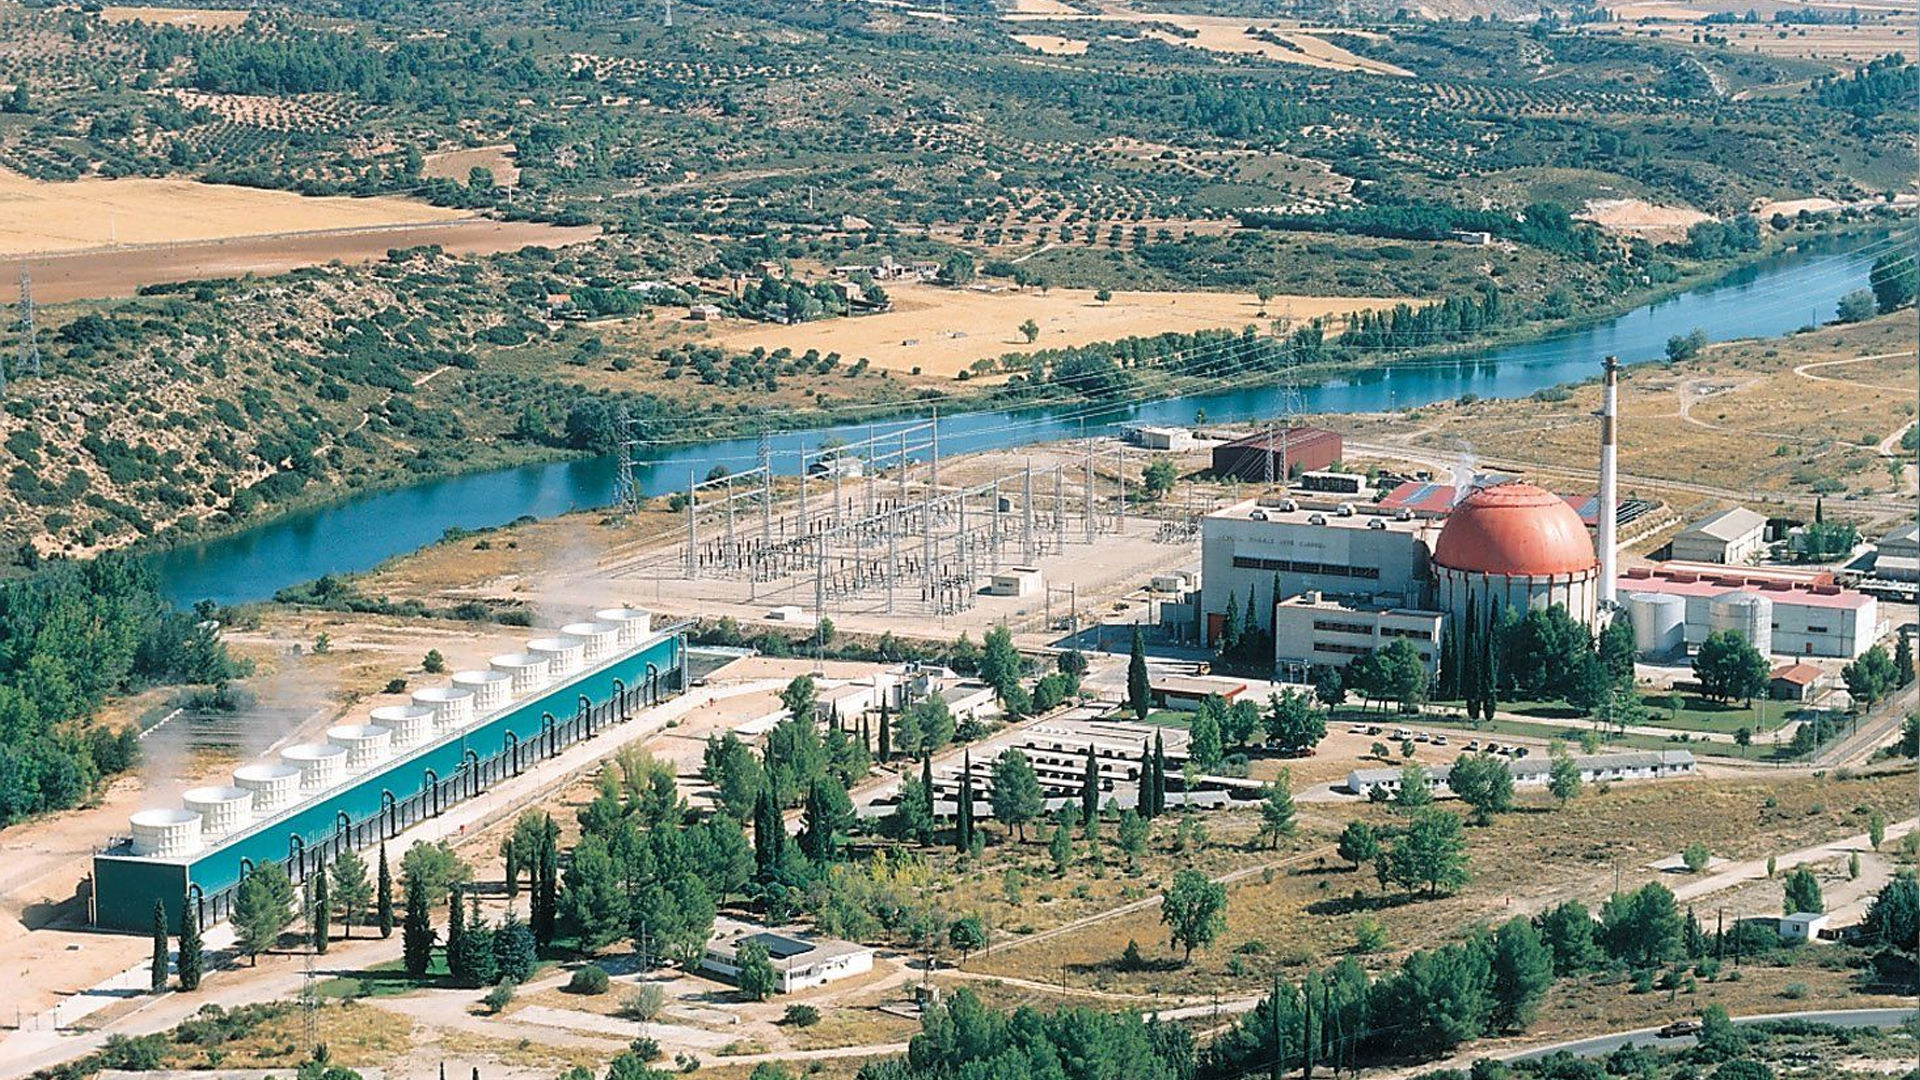
\includegraphics[width=0.85\textwidth]{content/figures/zorita.jpg}
    \caption{Central Nuclear José Cabrera (\cite{sne_recursos_prensa}).}
    \label{fig:zorita}
\end{figure}

El cese definitivo de explotación de la central fue declarado por el Ministerio de Industria, Turismo y Comercio mediante la Orden Ministerial del 20 de abril de 2006. El titular de las actividades de desmantelamiento de la central es \acrshort{enresa}, por lo que se tubo que cambiar la titularidad de la instalación de Gas Natural Fenosa a \acrshort{enresa}. El 11 de febrero de 2010, \acrshort{enresa} inició el desmantelamiento de la instalación.

La alternativa escogida fue un desmantelamiento total e inmediato en un horizonte temporal de unos ocho años. Las actividades de desmantelamiento comprenden también la segmentación mediante técnicas de corte especiales de grandes sistemas y componentes radiológicamente significativos, como el generador de vapor y la vasija del reactor, así como la descontaminación y demolición de edificios y la restauración final del emplazamiento. 

Actualmente, la instalación se encuentra en la fase de restauración, en la cual se pretende devolver al emplazamiento a sus condiciones previas a la construcción de la central, saneando todo el terreno en cuestión. Los elementos de combustible irradiado de la central se están almacenando temporalmente en el \acrfull{ati} de la instalación, en el que también se han depositado algunos residuos generados durante el desmantelamiento (\cite{enresa_desmantelamiento_zorita}).

En la siguiente tabla se resume lo más importante de lo expuesto anteriormente sobre la central nuclear de Zorita:

\begin{table}[!h]
    \resizebox{\textwidth}{!}{%
    \begin{tabular}{|cc|cl|cc|}
    \hline
    \rowcolor[HTML]{ECF4FF} 
    \multicolumn{2}{|c|}{\cellcolor[HTML]{ECF4FF}\textbf{Localización}} &
      \multicolumn{2}{c|}{\cellcolor[HTML]{ECF4FF}\textbf{Propiedad}} &
      \multicolumn{1}{c|}{\cellcolor[HTML]{ECF4FF}\textbf{Titular}} &
      \textbf{Tipo} \\ \hline
    \multicolumn{2}{|c|}{Almonacid de Zorita (Guadalajara)} & \multicolumn{2}{c|}{Unión Fenosa (Naturgy)} & \multicolumn{1}{c|}{Enresa}      & PWR    \\ \hline
    \rowcolor[HTML]{ECF4FF} 
    \multicolumn{1}{|c|}{\cellcolor[HTML]{ECF4FF}\textbf{Potencia térmica}} &
      \textbf{Potencia eléctrica} &
      \multicolumn{2}{c|}{\cellcolor[HTML]{ECF4FF}\textbf{Refrigeración}} &
      \multicolumn{2}{c|}{\cellcolor[HTML]{ECF4FF}\textbf{Autorización construcción}} \\ \hline
    \multicolumn{1}{|c|}{510 MWt}         & 150 MWe         & \multicolumn{2}{c|}{Abierta - Río Tajo}                & \multicolumn{2}{c|}{24 de junio de 1964}  \\ \hline
    \rowcolor[HTML]{ECF4FF} 
    \multicolumn{2}{|c|}{\cellcolor[HTML]{ECF4FF}\textbf{Autorización de puesta en marcha}} &
      \multicolumn{2}{c|}{\cellcolor[HTML]{ECF4FF}\textbf{Cese de explotación}} &
      \multicolumn{2}{c|}{\cellcolor[HTML]{ECF4FF}\textbf{Autorización desmantelamiento}} \\ \hline
    \multicolumn{2}{|c|}{11 de octubre de 1968}             & \multicolumn{2}{c|}{30 de abril de 2006}               & \multicolumn{2}{c|}{1 de febrero de 2010} \\ \hline
    \end{tabular}%
    }
    \caption{Características y fechas clave de la Central Nuclear José Cabrera (\cite{csn_info_zorita}).}
    \label{tabla:resumen_zorita}
    \end{table}

\newpage
\subsubsection{Comparación de la Central Nuclear de Zorita con el reactor AP300} \label{comparacion_zorita_ap300}

Llegados a este punto, se han expuesto detalladamente tanto las características del \acrshort{smr} AP300 como las de la Central Nuclear José Cabrera, por lo que se recogen a continuación las similitudes y diferencias entre ambas plantas:

\begin{table}[h]
  \centering
  \begin{tabular}{|
  >{\columncolor[HTML]{CBE5CB}}c |
  >{\columncolor[HTML]{FFCCC9}}c 
  >{\columncolor[HTML]{FFCCC9}}c |}
  \hline
  \cellcolor[HTML]{ECF4FF} &
    \multicolumn{2}{c|}{\cellcolor[HTML]{ECF4FF}\textbf{DIFERENCIAS}} \\ \cline{2-3} 
  \multirow{-2}{*}{\cellcolor[HTML]{ECF4FF}\textbf{SIMILITUDES}} &
    \multicolumn{1}{c|}{\cellcolor[HTML]{FFCE93}\textbf{AP300}} &
    \cellcolor[HTML]{FFCE93}\textbf{Central Nuclear de Zorita} \\ \hline
  \cellcolor[HTML]{CBE5CB}Tipo: \acrshort{pwr} &
    \multicolumn{1}{c|}{\cellcolor[HTML]{FFCCC9}\begin{tabular}[c]{@{}c@{}}Generación III+ \end{tabular}} &
    \begin{tabular}[c]{@{}c@{}}Entre generación I y II \end{tabular} \\ \hline
  \begin{tabular}[c]{@{}c@{}}Potencia eléctrica\\ propia de los \acrshortpl{smr} \\ (entre 10 y 300 MWe)\end{tabular} &
    \multicolumn{1}{c|}{\cellcolor[HTML]{FFCCC9}\begin{tabular}[c]{@{}c@{}}Potencia de 300 MWe\\ y 900 MWt\end{tabular}} &
    \begin{tabular}[c]{@{}c@{}}Potencia de 150 MWe\\ y 510 MWt\end{tabular} \\ \hline
  Diseño Westinghouse &
    \multicolumn{1}{c|}{\cellcolor[HTML]{FFCCC9}\begin{tabular}[c]{@{}c@{}}Ciclos de operación\\ de 4 años\end{tabular}} &
    \begin{tabular}[c]{@{}c@{}}Ciclos de operación\\ de 15 meses\end{tabular} \\ \hline
  \begin{tabular}[c]{@{}c@{}}Combustible: Uranio\\ de bajo \\ enriquecimiento\end{tabular} &
    \multicolumn{1}{c|}{\cellcolor[HTML]{FFCCC9}\begin{tabular}[c]{@{}c@{}}Elementos de combustible\\ de $12 \times 12$ varillas\end{tabular}} &
    \begin{tabular}[c]{@{}c@{}}Elementos de combustible\\ de $14 \times 14$ varillas\end{tabular} \\ \hline
  \cellcolor[HTML]{CBE5CB} &
    \multicolumn{1}{c|}{\cellcolor[HTML]{FFCCC9}\begin{tabular}[c]{@{}c@{}}Sistemas de seguridad \\ mayoritariamente pasivos\end{tabular}} &
    \begin{tabular}[c]{@{}c@{}}Sistemas de seguridad\\ dependientes de \\ alimentación eléctrica \\ exterior\end{tabular} \\ \cline{2-3} 
  \cellcolor[HTML]{CBE5CB} &
    \multicolumn{1}{c|}{\cellcolor[HTML]{FFCCC9}\begin{tabular}[c]{@{}c@{}}Edificio del reactor\\ ultracompacto, con el \\ tanque del sistema de \\ enfriamiento pasivo de \\ la contención en la parte \\ superior del mismo \\ (ver figura \ref{fig:ap300_inside_nsss})\end{tabular}} &
    \begin{tabular}[c]{@{}c@{}}Edificio de contención \\ característico, con una cúpula \\ hemisférica de acero\\ (ver figura \ref{fig:zorita})\end{tabular} \\ \cline{2-3} 
  \multirow{-3}{*}{\cellcolor[HTML]{CBE5CB}1 solo lazo} &
    \multicolumn{1}{c|}{\cellcolor[HTML]{FFCCC9}\begin{tabular}[c]{@{}c@{}}Capacidades avanzadas \\ de seguimiento de carga\\  con tasas de potencia\\ del $\pm 5\%/min$\end{tabular}} &
    \begin{tabular}[c]{@{}c@{}}Diseñado para operar\\ fundamentalmente a \\ potencia nominal, \\ con capacidades de \\ variación de potencia \\ del $\pm 3\%/min$\end{tabular} \\ \hline
  \end{tabular}
  \caption{Tabla comparativa de las similitudes y diferencias más importantes entre el AP300 y la Central Nuclear de Zorita.}
  \label{tab:comparacion_ap300_zorita}
  \end{table}

En resumen, puede observarse que la central nuclear de Zorita presenta muchas características idénticas o muy similares al AP300. Aun así, la principal diferencia entre ambas tecnologías radica en la generación o época de implementación de cada una. Esto último conlleva una importante desactualización por parte de la central nuclear de Zorita con respecto al diseño, los materiales, los sistemas de seguridad, protección y control avanzados que tiene el AP300.

Es importante destacar que ambas centrales presentan unas tasas de variación de potencia muy similares, aunque ---a diferencia de Zorita--- el AP300 se ha diseñado intencionadamente para realizar seguimiento de carga, por lo que está más preparado para operar en este modo de forma adecuada.

\subsubsection{El Simulador Gráfico Interactivo de Zorita (SGIZ)} \label{sgiz}

El \acrshort{sgiz} es un simulador gráfico interactivo de alcance total en tiempo real de la Central Nuclear de Zorita. Durante los años de operación de la central, se empleó para el entrenamiento de los operadores de la sala de control, para comprender y analizar la dinámica de la planta y para desarrollar y validar sus procedimientos operativos de emergencia.

En abril de 2008 se firmó el convenio de colaboración entre Unión Fenosa y la UPM para la creación del Aula ``José Cabrera'', donde se instaló el \acrshort{sgiz}. Este aula se ubica en el Departamento de Ingeniería Nuclear de la ETSII-UPM y está dedicada a la enseñanza de la tecnología de la operación de las centrales nucleares.

El simulador proporciona las respuestas de la planta durante la operación normal, transitorios y condiciones de accidente, basadas en el código \acrshort{trac} y un conjunto de pantallas ilustrativas en tiempo real, así como un conjunto de alarmas en un panel similar al de la sala de control real de la central nuclear, permitiendo la operación automática y manual en tiempo real de los componentes del sistema completo tanto en condiciones normales como de emergencia.

Existen tres modos de simulación en el \acrshort{sgiz}:

\begin{enumerate}
  \item \textbf{Modo de ejecución a tiempo real con alarmas activadas:} Es el modo de operación más empleado, ya que se ajusta a los períodos reales en los que suceden los distintos acontecimientos en la operación de la central.
  \item \textbf{Modo de ejecución a tiempo real sin alarmas:} Las alarmas pueden observarse en la pantalla de ``alarmas'' de la simulación, pero el panel con sus respectivas bocinas se encuentra desactivado. Es un modo de operación adecuado para experiencias ya conocidas en las que se quiere prescindir de la molestia que puede provocar el ruido de las alarmas.
  \item \textbf{Modo de ejecución rápido (FAST) sin alarmas:} El código se ejecuta a una velocidad muy superior al tiempo real, en concreto, 20 veces más rápido. Resulta especialmente útil para simulaciones de larga duración.
\end{enumerate}


\begin{figure}[!h]
  \centering
  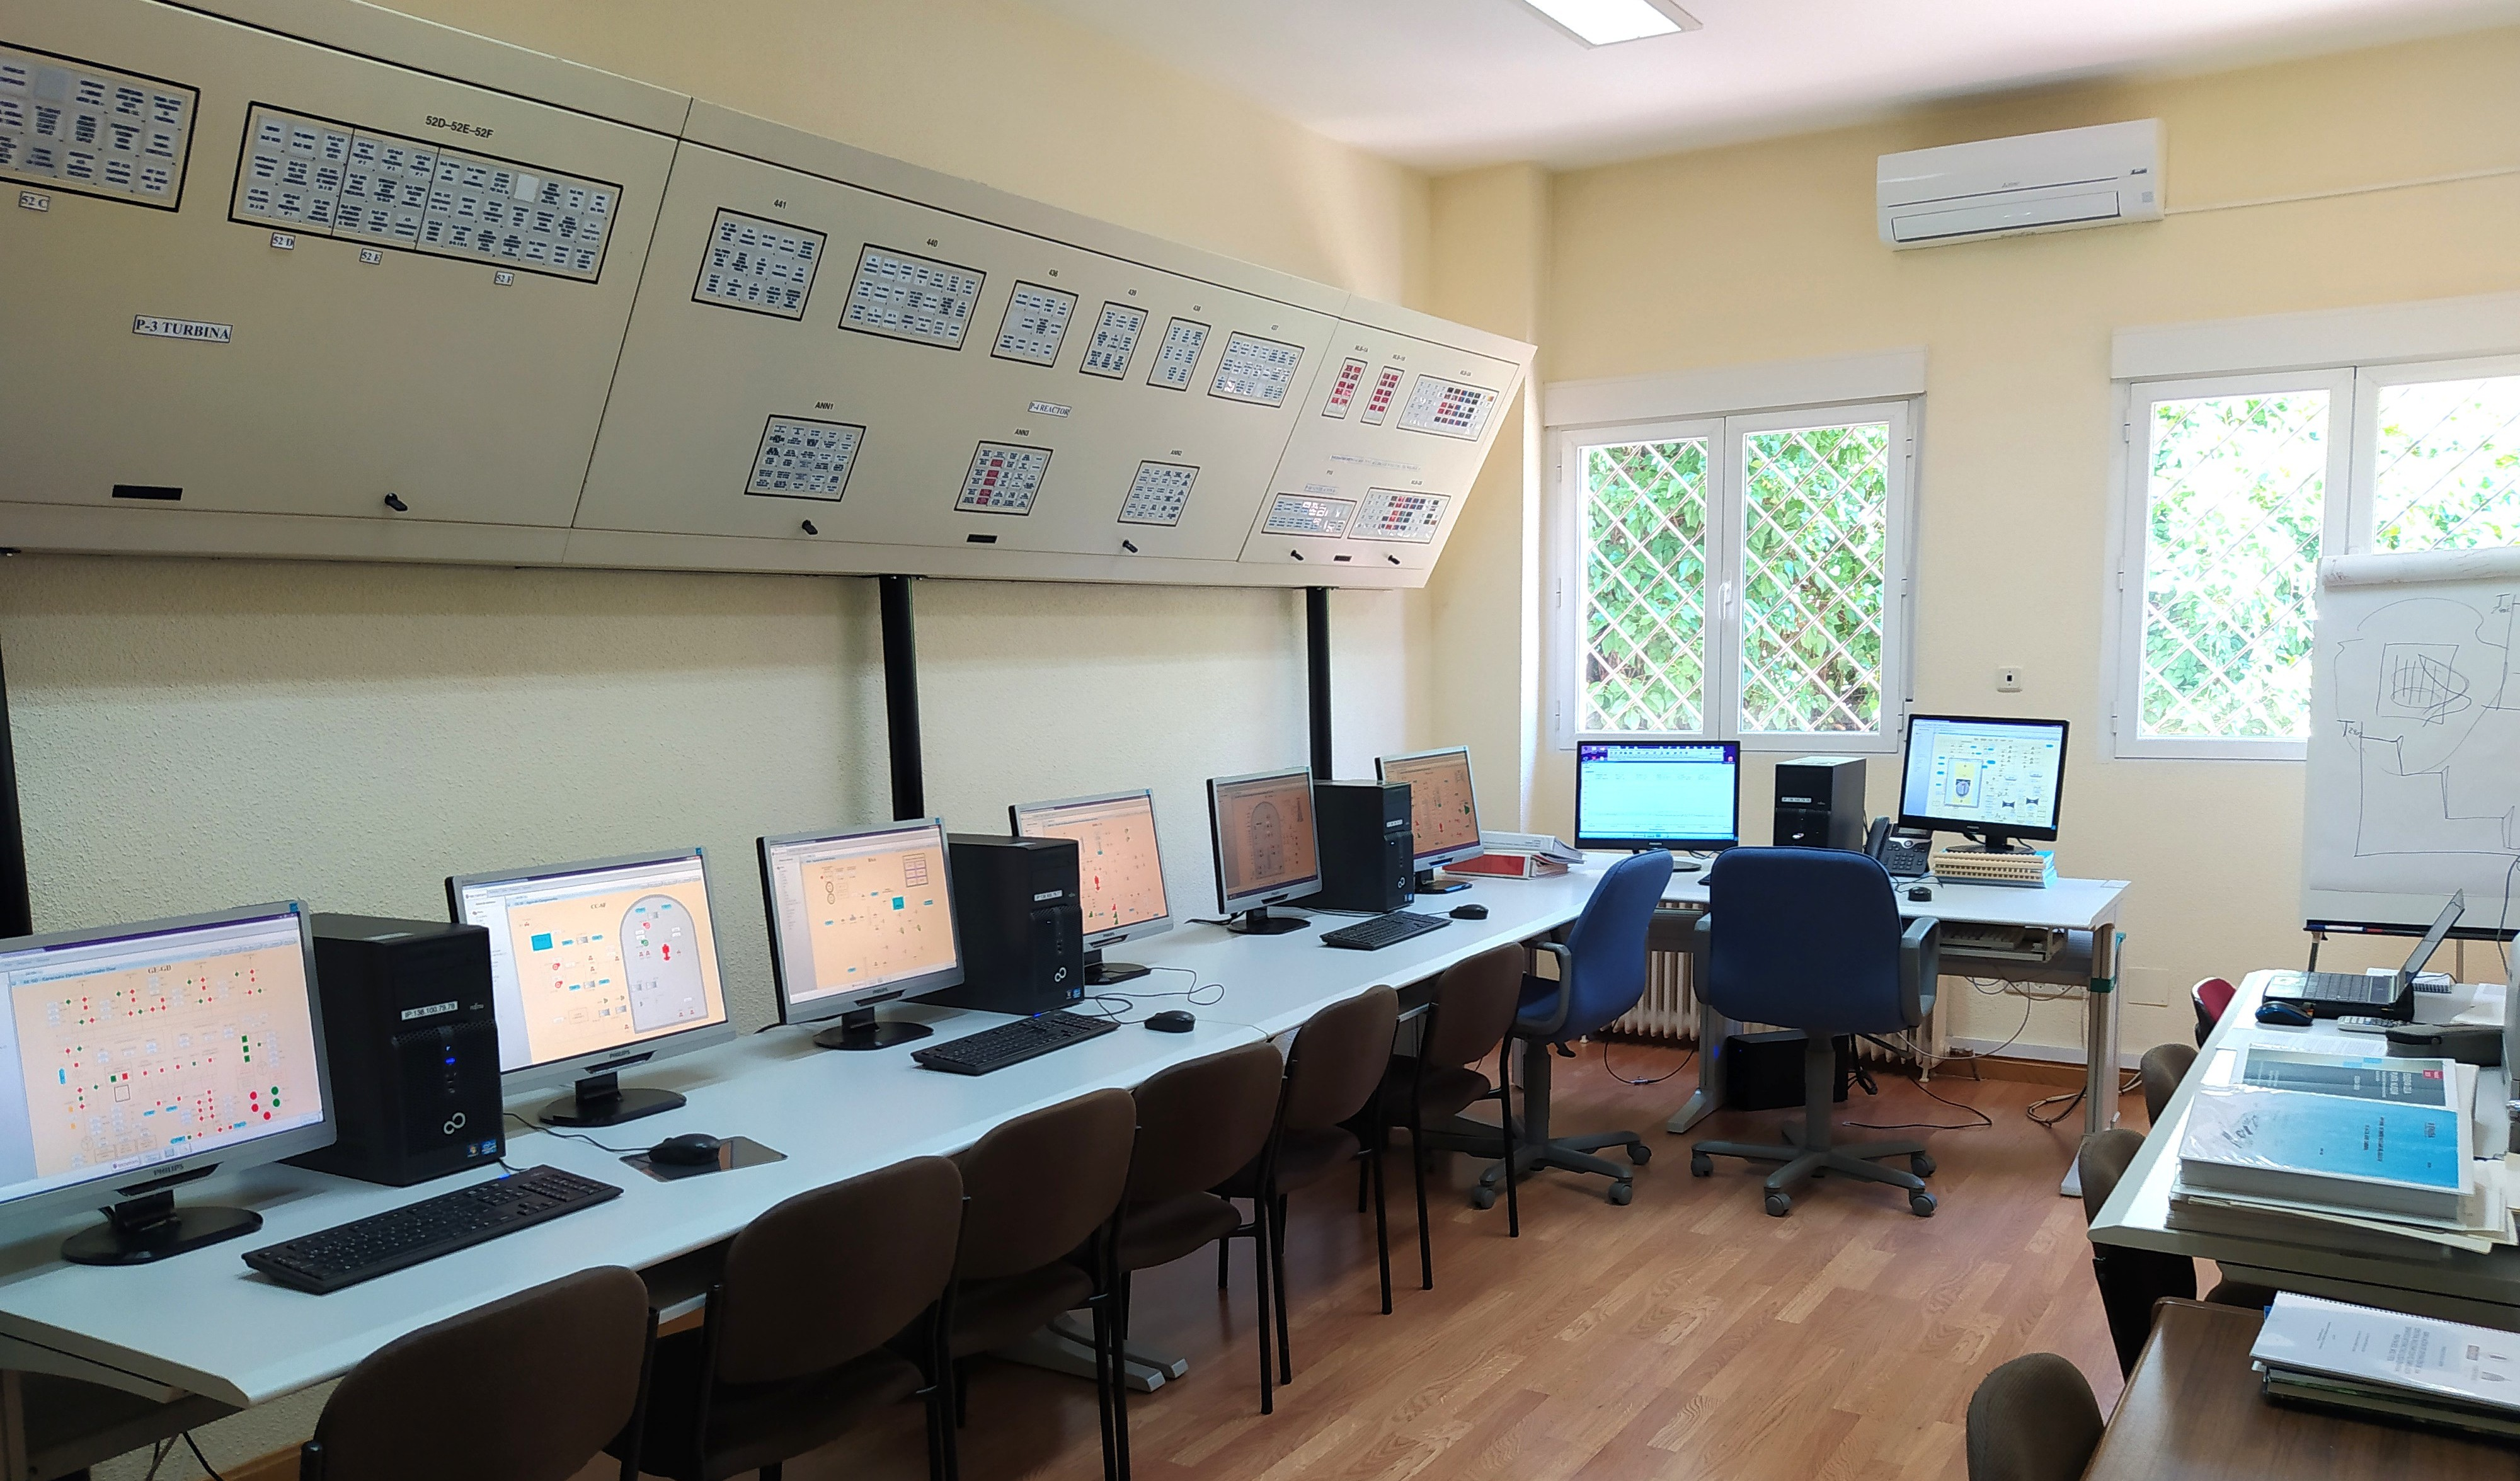
\includegraphics[width=0.8\textwidth]{content/figures/sgiz.jpg}
  \caption{Simulador Gráfico Interactivo de Zorita (ETSII - UPM).}
  \label{fig:sgiz}
\end{figure}